% paper/sections/06_discussion.tex
% Prose for §6. Outline: paper/06_discussion.md.
% Five subsections; 0.5 pg target / 0.75 pg ceiling.
%
%   §6.1 Path-cost: edit friction on Claude SWE-bench   (sec:disc-pathcost)
%   §6.2 Pricing asymmetry: batching + output-control   (sec:disc-pricing)
%   §6.3 Failure-cost + capability invariance           (sec:disc-failurecost)
%   §6.4 Where the method works / doesn't               (sec:disc-scope)
%   §6.5 Implications for agent design                  (sec:disc-design)
%
% Numbers resolve through \result / \resp / \respct macros backed by CSVs
% in paper/data/.

% (Section heading and \label{sec:discussion} come from main.tex.)

% ─────────────────────── §6.1 — path-cost / edit friction ──────────────
\subsection{Path-cost: edit friction on Claude SWE-bench}
\label{sec:disc-pathcost}
\label{sec:discussion-edit-friction}
The lone cell of Table~\ref{tab:code-only-headline} in which
\texttt{code\_only} is directionally costlier than its rival is Claude
$\times$ SWE-bench: cost runs $+14\%$ (NS) but output tokens are $+40\%$
at $p{<}10^{-9}$---the extra cost scales with output volume rather than
reflecting a fixed per-run overhead. The
working hypothesis is edit friction: under \texttt{code\_only}, every
file modification must be expressed as a Python script rather than as a
single native \texttt{Edit} or \texttt{Write} call. The per-instance
Spearman correlation between $\Delta_{\text{edit chars}}$
(\texttt{code\_only} $-$ \texttt{baseline}, computed from JSONL tool-use
blocks) and $\Delta_{\text{output tokens}}$ is
$\rho = \result{edit_friction}{rho_edit_chars:value}[2]$
($p = \resp{edit_friction}{rho_edit_chars_p:value}$,
$n = \result{edit_friction}{n_instances:value}[0]$); a median split confirms
that the per-instance penalty scales with edit volume, with
$\Delta_{\text{output tokens}} =
\result{edit_friction}{lowpatch_delta_output_tokens:value}[0]$ on the
low-patch half vs.\
$\result{edit_friction}{highpatch_delta_output_tokens:value}[0]$ on the
high-patch half (one-sided Mann--Whitney
$p = \resp{edit_friction}{highpatch_mw_p:value}$). About
$\result{edit_friction}{intercept_gap:value}[0]$ tokens of the aggregate gap
is fixed-cost regime verbosity (OLS intercept at zero patch size); edit
friction is the additional per-line tax, not the whole gap.

% ─────────────────────── §6.2 — pricing asymmetry ──────────────────────
\subsection{Pricing asymmetry: batching and programmatic output control on Codex}
\label{sec:disc-pricing}
\label{sec:discussion-codex-batching}

\begin{figure}[t]
\centering
% paper/figures_src/03_batching.tikz.tex
%
% Figure 3 — H1 tool-call batching case study (sphinx-doc__sphinx-7757,
% Codex, seed 3, both arms PASS). Structural mockup of one LLM step.
%
% Top panel (baseline arm): one assistant turn followed by three parallel
% exec_command tool calls — agent gathers context with three independent
% lookups.
%
% Bottom panel (code-only arm): same assistant turn followed by a single
% execute_code call bundling the same three lookups into one script.
%
% Intent-only labels (per Design decision §6 of figures_outline.md): cards
% carry the *purpose* of each lookup, not the literal command. File names
% appear as small grey subtitles for grounding only. No regex / Python
% source.
%
% Wrapped inside a \begin{figure}...\end{figure} float in
% sections/06_discussion.tex. main.tex must load \usepackage{tikz} +
% \usetikzlibrary{positioning,fit,backgrounds,arrows.meta}.

{% local scope for the inline-formatting commands
\providecommand{\toolhdr}[1]{{\footnotesize\sffamily\bfseries\color{black!75}#1}}
\providecommand{\intent}[1]{{\footnotesize #1}}
\providecommand{\subtitle}[1]{{\scriptsize\ttfamily\color{black!55}#1}}

\begin{tikzpicture}[
  font=\small,
  every node/.style={inner sep=2pt},
  bubble/.style={
    draw=black!50, line width=0.4pt,
    rounded corners=2pt,
    fill=black!4,
    text width=0.78\columnwidth,
    align=left,
    inner sep=4pt,
    font=\footnotesize\itshape,
  },
  toolcard/.style={
    draw=black!70, line width=0.5pt,
    rounded corners=3pt,
    text width=0.62\columnwidth,
    align=left,
    inner sep=4pt,
  },
  bundlecard/.style={
    draw=black!70, line width=0.7pt,
    rounded corners=3pt,
    text width=0.74\columnwidth,
    align=left,
    inner sep=5pt,
    fill=black!2,
  },
  armtag/.style={font=\footnotesize\sffamily\bfseries, text=black!80},
  arrow/.style={->, >=stealth, line width=0.4pt, draw=black!55},
  node distance=3pt and 0pt,
]

% =========================================================================
% TOP PANEL — baseline arm (3 parallel exec_command calls)
% =========================================================================
\node[armtag] (baseTag) at (0, 0)
  {Baseline arm \,---\, 1 LLM step \, $\rightarrow$ \, 3 tool calls};

\node[bubble, below=4pt of baseTag, anchor=north] (baseBubble)
  {Assistant: I need to see the definition, an existing test, and how
   it's called elsewhere.};

\node[toolcard, below=6pt of baseBubble.south west, anchor=north west]
  (b1) {%
    \toolhdr{exec\_command}\\
    \intent{read definition site}\\
    \subtitle{sphinx/domains/python.py}%
  };
\node[toolcard, below=3pt of b1.south west, anchor=north west]
  (b2) {%
    \toolhdr{exec\_command}\\
    \intent{read existing test}\\
    \subtitle{tests/test\_util\_inspect.py}%
  };
\node[toolcard, below=3pt of b2.south west, anchor=north west]
  (b3) {%
    \toolhdr{exec\_command}\\
    \intent{search call sites}\\
    \subtitle{tests/}%
  };

% Faint left "bracket" to suggest the three are parallel
\draw[arrow] (baseBubble.south) -- ++(0, -0.18);
\draw[black!40, line width=0.4pt]
  ([xshift=-6pt]b1.north west) -- ([xshift=-6pt]b3.south west);
\draw[black!40, line width=0.4pt]
  ([xshift=-6pt]b1.north west) -- ([xshift=-3pt]b1.north west);
\draw[black!40, line width=0.4pt]
  ([xshift=-6pt]b3.south west) -- ([xshift=-3pt]b3.south west);

% Divider between panels
\draw[black!25, line width=0.4pt, dashed]
  ([yshift=-10pt]b3.south west) -- ++(\columnwidth, 0);

% =========================================================================
% BOTTOM PANEL — code-only arm (1 execute_code call bundling all three)
% =========================================================================
\node[armtag, below=14pt of b3.south west, anchor=north west] (coTag)
  {Code-only arm \,---\, 1 LLM step \, $\rightarrow$ \, 1 tool call};

\node[bubble, below=4pt of coTag.south west, anchor=north west] (coBubble)
  {Assistant: I need to see the definition, an existing test, and how
   it's called elsewhere.};

\node[bundlecard, below=6pt of coBubble.south, anchor=north]
  (co1) {%
    \toolhdr{execute\_code} \, \subtitle{one script}\\[2pt]
    \intent{$\bullet$\, read definition site} \hfill \subtitle{sphinx/domains/python.py}\\
    \intent{$\bullet$\, read existing test} \hfill \subtitle{tests/test\_util\_inspect.py}\\
    \intent{$\bullet$\, search call sites} \hfill \subtitle{tests/}%
  };

\draw[arrow] (coBubble.south) -- (co1.north);

\end{tikzpicture}
}% end local scope

\caption{Tool-call batching at one LLM step
(Codex on \texttt{sphinx-doc\allowbreak\_\_sphinx-7757}; both arms PASS). On a
context-gathering step, the baseline arm emits three parallel
\texttt{exec\_command} calls; the code-only arm bundles the same three
lookups into a single \texttt{execute\_code} script. The aggregate ratio
of tool calls per LLM call is $1.35$ (baseline) vs.\ $0.89$ (code-only)
on Codex SWE-bench.}
\label{fig:batching-case}
\end{figure}

\begin{figure}[t]
\centering
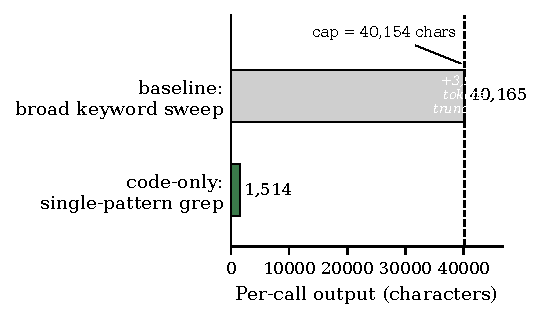
\includegraphics[width=\columnwidth]{generated/figures/04_h2_truncation}
\caption{Per-call output at one LLM step
(Codex on \texttt{django\allowbreak\_\_django-11848}; both arms PASS). The baseline
arm's broad keyword sweep matched unrelated fixture data and pinned the
\texttt{exec\_command} output cap at
$\result{fig.04_h2_truncation}{exec_command_cap}$~chars
($+\result{fig.04_h2_truncation}{truncation_tokens}$~tokens elided);
the code-only arm's narrower scope returned
$\result{fig.04_h2_truncation}{onlycode_chars}$~chars cleanly. The
aggregate $p99$ collapse in \S\ref{sec:disc-pricing} is the
population-level analogue of this case.}
\label{fig:truncation-case}
\end{figure}

Why does Codex's \texttt{code\_only} save ${\sim}25\%$ on input tokens
on SWE-bench while LLM-call counts stay essentially flat
($\result{mcp_output_size}{codex_swebench:baseline:llm_calls_per_run}$
for \texttt{baseline} vs.\
$\result{mcp_output_size}{codex_swebench:onlycode:llm_calls_per_run}$
for \texttt{code\_only})? Two mechanisms, neither reproduced by the
\texttt{bash\_only} control, jointly drive the win. \emph{Tool-call
batching:} \texttt{execute\_code} issues
$\result{mcp_output_size}{codex_swebench:onlycode:calls_per_run}$ tool
calls per run vs.\
$\result{mcp_output_size}{codex_swebench:baseline:calls_per_run}$ for
\texttt{baseline}, so a single Python script subsumes what
\texttt{exec\_command} requires several calls to do
(Figure~\ref{fig:batching-case} shows one such step on a named
instance). \emph{Upper-tail
suppression:} median per-call output is essentially
unchanged
($\result{mcp_output_size}{codex_swebench:onlycode:median_chars}[0]$
vs.\
$\result{mcp_output_size}{codex_swebench:baseline:median_chars}[0]$
chars), but the $p99$ collapses from the \texttt{exec\_command} ceiling
of $\result{mcp_output_size}{codex_swebench:baseline:p99_chars}[0]$
chars to
$\result{mcp_output_size}{codex_swebench:onlycode:p99_chars}[0]$---the
agent constrains per-call output volume programmatically, by tightening
query scope, slicing returned text, or staging output across multiple
prints, rather than receiving whatever the native tool emits
(Figure~\ref{fig:truncation-case} catches the cap-pinning event on a
named instance). This refines the industry token-reduction
claim~\cite{blog:anthropic2025codemcp,blog:cloudflare2025codemode}: the
gain materialises when the agent's API expresses per-call batching
\emph{and} its native rival exposes a hard output ceiling, not from the
\texttt{execute\_code} surface alone. Claude's API empirically does not
batch on SWE-bench (\texttt{code\_only} issues
$\result{mcp_output_size}{claude_swebench:onlycode:calls_per_run}$
calls per run vs.\
$\result{mcp_output_size}{claude_swebench:baseline:calls_per_run}$ for
\texttt{baseline}), and the round-count inflation is the input-token
mirror of the edit-friction effect in \S\ref{sec:disc-pathcost}---one
mechanism viewed at two granularities.

% ─────────────────────── §6.3 — failure-cost / capability ──────────────
\subsection{Failure-cost and capability invariance}
\label{sec:disc-failurecost}
\label{sec:discussion-failure-cost}
Pass rates differ by less than three percentage points across every cell
while costs swing $20$--$40\%$ (Table~\ref{tab:code-only-headline}). The
straightforward interpretation is that tool restriction is a harness-efficiency axis
orthogonal to model capability: the model solves the task with any
reasonable interface; the surface changes the path, not the answer.
This matches the Capability Overlap
Principle~\cite{zhang2026tooltax} and the pass-rate invariance
reported under tool ablation in~\cite{report:verdent2025swebench}. The
agreement matrix (Table~\ref{tab:agreement-matrix}) confirms it:
unanimous-outcome instances dominate every cell at
${\geq}\result{agreement_matrix}{_all:_all:min_unanimous_majority_pct}[0]\%$
under majority vote and
${\geq}\result{agreement_matrix}{_all:_all:min_unanimous_strict_pct}[0]\%$
on the strictest $9/9$-trials criterion. The Claude $\times$ SWE-bench
cost gap decomposes cleanly against this anchor
(Table~\ref{tab:headline-unanimous}): on the unanimous-pass subset
$\Delta_{\text{cost adj.}}$ collapses from
$+\result{headline_unanimous}{swebench:claude:onlycode-vs-baseline:cost_adj:full_mean_delta_pct}[1]\%$
to
$+\result{headline_unanimous}{swebench:claude:onlycode-vs-baseline:cost_adj:unanimous_majority_mean_delta_pct}[1]\%$
(NS), $\Delta_{\text{input tokens}}$ from
$+\result{headline_unanimous}{swebench:claude:onlycode-vs-baseline:input_tokens:full_mean_delta_pct}[1]\%$
to
$+\result{headline_unanimous}{swebench:claude:onlycode-vs-baseline:input_tokens:unanimous_majority_mean_delta_pct}[1]\%$
(NS), but $\Delta_{\text{output tokens}}$ stays at
$+\result{headline_unanimous}{swebench:claude:onlycode-vs-baseline:output_tokens:unanimous_majority_mean_delta_pct}[1]\%$
(highly significant). Two mechanisms cohabit the cell: the
\S\ref{sec:disc-pathcost} edit-friction path-cost is the output-side
tax that persists on successful runs; the remaining input-side
blow-up is a failure-cost---extended doomed-run trajectories on
instances no surface can solve. Conditioning on success separates them.
The cache-floor median is byte-identical on subset and full set in
$\result{agreement_matrix}{_all:_all:cache_floor_unchanged_majority}[0]$
of $\result{agreement_matrix}{_all:_all:cache_floor_total_groups}[0]$
(benchmark, seed, agent, arm) groups (\S\ref{sec:method-cost}), so the
collapse is not a cost-adjustment artefact.

% ─────────────────────── §6.4 — scope of the method ───────────────────
\subsection{Where the method works, and where it does not}
\label{sec:disc-scope}
The harness quantifies tool-surface tax under cache noise
(\S\ref{sec:method-cost}), isolates regime effects via the
artifact-vs-SWE-bench split, and surfaces agent-design coupling: the
same restriction (\texttt{code\_only}) produces a significant cost win
for Codex on SWE-bench ($p{<}10^{-8}$) and a non-significant
directionally-costlier result for Claude in the same cell --- the
sharpest \emph{agent-design} contrast in the four-cell structure. It
does not support model-capability claims, because pass rates are
statistically tied; the path-vs-answer dissociation in
\S\ref{sec:disc-failurecost} licenses the cost contrasts as
cost-engineering rather than capability claims. We make no per-repo
SWE-bench claims at $n{\approx}12$--$15$; the remaining headline
caveat is the NS Claude $\times$ SWE-bench cell at $p{\approx}0.12$.

% ─────────────────────── §6.6 — implications for design ────────────────
\subsection{Implications for agent design}
\label{sec:disc-design}
The four-cell structure adjudicates between the prior prescriptions of
\S\ref{sec:introduction} as follows. \emph{Computation-dominated
workloads:} drop the IDE surface; \texttt{code\_only} wins on cost at
parity capability (Artifact $\times$ Claude, Table~\ref{tab:code-only-headline}).
\emph{Modification-dominated workloads with a high solve-rate:} the
surface choice is roughly cost-neutral on Claude---the headline
$+\result{headline_unanimous}{swebench:claude:onlycode-vs-baseline:cost_adj:full_mean_delta_pct}[1]\%$
penalty is a failure-cost effect on doomed runs, not a per-edit tax on
successful ones (Table~\ref{tab:headline-unanimous}).
\emph{Modification-dominated workloads with a low solve-rate:} keep
\texttt{Edit} and \texttt{Write} at minimum---the edit-friction
path-cost in \S\ref{sec:disc-pathcost} compounds with the failure-cost
in \S\ref{sec:disc-failurecost} on instances no surface can solve.
\emph{Tool surfaces that admit batching and programmatic output control:} expect
input-token savings of the kind Codex realises in
\S\ref{sec:disc-pricing}, provided the workload does not push LLM-call
count up in the process.
